\chapter{Approximating the Calcium Concentration}
\label{chapter:approximating}

If we have a look at the typical trajectory of the calcium concentration in activated and unactivated cells, shown in figure~\ref{fig:all_cells_overlayed}, we can see differences emerging. For one the maximum concentration value reached by most activated cells is higher. Another distinguishing feature is the presence of a steep incline at the moment of activation.

\begin{figure}
	\centering
	\begin{subfigure}{0.45\linewidth}
		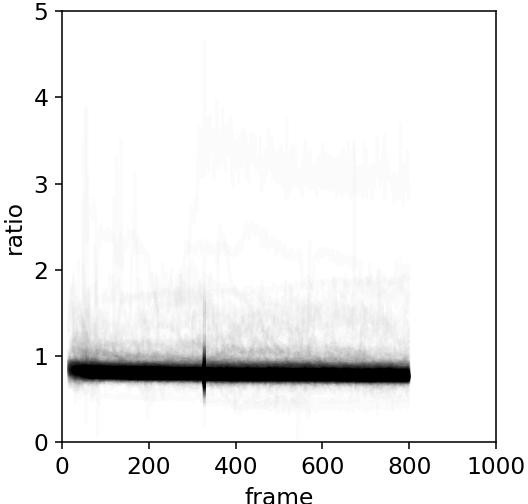
\includegraphics[width=\textwidth]{fig/all_cells_overlayed_mouse_neg}
	\end{subfigure}
	\hfill
	\begin{subfigure}{0.45\linewidth}
		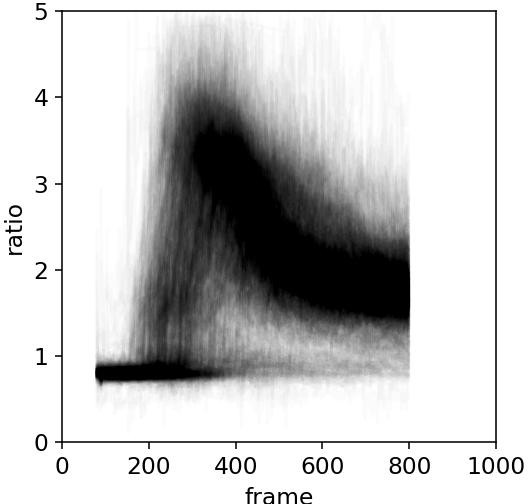
\includegraphics[width=\textwidth]{fig/all_cells_overlayed_mouse_pos}
	\end{subfigure}
	
	\caption{Two plots of the overlapping calcium concentration time series of cells. On the left a negative control and on the right a positive control of mouse cells.}
	\label{fig:all_cells_overlayed}
\end{figure}

By modelling the time series with a function incorporating features such as the increase, maximum value and oscillations present in the decrease afterwards, we can extract these features more easily. By doing this, using approximation methods from chapter~\ref{chapter:optimization}, we want to answer the research questions from the introduction.

From studying the data in the two control groups we find to expect a function close to
\begin{align}
	\label{math:function_unactivated_cell}
	f_{unac}(x) := u
\end{align}
for unactivated cells and
\begin{align}
	\label{math:function_activated_cell}
	f_{ac}(x) := \begin{cases}
		\frac{a-u}{1 + e^{-k_1(x-w_1)}} + u & \textbf{ if } x <= t\\
		\frac{a-d}{1 + e^{-k_2(x-w_2)}} + d & \textbf{ else}
	\end{cases}
\end{align}
for activated cells. The parameters can be understood as described in table~\ref{tab:parameters}.

\begin{table}[h!]
	\centering
	\begin{tabular}{|cl|}
		\hline
		$u$ ... & average value before activation, \\
		\hline
		$a$ ... & value reached at the peak of activation, \\
		\hline
		$d$ ... & average value after activation, \\
		\hline
		$k_1$ ... & steepness of increase, \\
		\hline
		$k_2$ ... & steepness of decrease, \\
		\hline
		$w_1$ ... & time point at which the increase happens, \\
		\hline
		$w_2$ ... & time point at which the decrease happens, \\
		\hline
		$t$ ... & time point at which the increase ends, and the decrease starts, \\
		\hline
	\end{tabular}
	\label{tab:parameters}
	\caption{List of parameters and their interpretation.}
\end{table}

Figure~\ref{fig:typical_time_series_with_parameters} shows how the above functions~\ref{math:function_unactivated_cell} and~\ref{math:function_activated_cell} look and how the relations to the parameters are in unactivated and activated cells.

% start = 50, u = 0.9, a = 4, k1 = 0.075, k2 = -0.04, w1 = 300, w2 = 520, t = 400, d = 2, z = 800

\begin{figure}
	\centering
	\begin{subfigure}{0.45\linewidth}
	  \begin{tikzpicture}
		\datavisualization [scientific axes, visualize as line,
			x axis = {
				min value = 0,
				max value = 1000,
				length = 5cm,
				ticks and grid = {major={at={0 as $t$}}, color=white},
				label = frame
			},
			y axis = {
				min value = 0,
				max value = 5,
				length = 5cm,
				ticks and grid = {major={at={0.9 as $u$}}},
				label = ratio
			},
		]
		data [format=function] {
			var x : interval [50:800]; func y = 0.9;
		};
	\end{tikzpicture}
	\end{subfigure}
	\hfill
	\begin{subfigure}{0.45\linewidth}
		\begin{tikzpicture}
			\datavisualization [scientific axes, visualize as line,
			x axis = {
				min value = 0,
				max value = 1000,
				length = 5cm,
				ticks and grid = {major={at={300 as $w_1$, 400 as $t$, 520 as $w_2$}}},
				label = frame
			}, y axis = {
				min value = 0,
				max value = 5,
				length = 5cm,
				ticks and grid = {major={at={0.9 as $u$, 2 as $d$, 4 as $a$}}},
				label = ratio
			},
			]
			data [separator=\space] {
				x y
				50 0.9000000223018123
				60 0.9000000472129365
				70 0.9000000999497857
				80 0.9000002115936903
				90 0.9000004479438116
				100 0.9000009482969035
				110 0.9000020075438745
				120 0.9000042499673413
				130 0.9000089971671542
				140 0.9000190469412669
				150 0.9000403220982461
				160 0.9000853606424553
				170 0.9001807029235496
				180 0.9003825231855573
				190 0.9008096899891967
				200 0.9017136137744631
				210 0.9036254818216721
				220 0.9076651317855678
				230 0.9161823896500311
				240 0.9340595221548389
				250 0.9712298467210794
				260 1.047020206850457
				270 1.1955833411872394
				280 1.4655191237997047
				290 1.8945460325562817
				300 2.45
				310 3.005453967443718
				320 3.434480876200295
				330 3.704416658812761
				340 3.8529797931495433
				350 3.9287701532789203
				360 3.9659404778451615
				370 3.983817610349969
				380 3.9923348682144324
				390 3.9963745181783277
				400 3.998286386225537
				410 3.9757431300314514
				420 3.964027580075817
				430 3.946806012846268
				440 3.9216685544064713
				450 3.8853516482022625
				460 3.8336546070121553
				470 3.7615941559557644
				480 3.664036770267849
				490 3.537049566998035
				500 3.379948962255225
				510 3.197375320224904
				520 3.0
				530 2.802624679775096
				540 2.620051037744775
				550 2.4629504330019647
				560 2.335963229732151
				570 2.238405844044235
				580 2.1663453929878447
				590 2.1146483517977375
				600 2.0783314455935287
				610 2.053193987153732
				620 2.035972419924183
				630 2.0242568699685486
				640 2.0163251423063198
				650 2.010972597798901
				660 2.007368479798872
				670 2.0049452463132695
				680 2.0033176021603487
				690 2.0022250720657206
				700 2.0014920576676736
				710 2.001000402214159
				720 2.0006707002609327
				730 2.0004496335404665
				740 2.0003014207161196
				750 2.0002020583878157
				760 2.0001354482992397
				770 2.000090795737405
				780 2.0000608631138013
				790 2.00004079817456
			}
			info {
			\draw (visualization cs: x=300, y=2.5)
			node [left,font=\footnotesize] {$k_1$};
			\draw (visualization cs: x=520, y=3.1)
			node [right,font=\footnotesize] {$k_2$};
			};
		\end{tikzpicture}
	\end{subfigure}
	
	\caption{Left shows the function $f_{unac}$ defined in~\ref{math:function_unactivated_cell} with the parameter $u$. The right shows the function $f_{ac}$ defined in~\ref{math:function_activated_cell} with the parameters $u$, $d$, $a$, $w_1$, $t$, $w_2$, $k_1$ and $k_2$.}
	\label{fig:typical_time_series_with_parameters}
\end{figure}

For our model to make sense we have to impose some conditions onto the parameters. We expect $0 \leq u \leq d \leq a$, $w_1 \leq t \leq w_2$, $k_1 > 0$ and $k_2 < 0$.

There are multiple ways in which the parameters of $f_{ac}$ can be chosen to get a function similar to $f_{unac}$. If $w_1$ is very large or $u \approx d \approx a$ then $f_{ac}$ approaches a constant value of $u$, thus approximating $f_{unac}$. If the approximation of a cell has parameters with $w_1$ very large or $u \approx d \approx a$ we can therefore expect it to be of an unactivated cell. Otherwise, it is more probable to be activated.

\section{Implementation}

Now that we have defined our model functions we will implement a routine that fits such a $f_{ac}$-function through the data of a cell.

First we describe a routine which handles reading the data, some necessary preprocessing steps and saving of the resulting parameter lists. The approximation itself is wrapped in the function \texttt{particle\_to\_parameters}, which takes a (frame, ratio)-matrix and returns a parameter list.

\begin{algorithm}[H] \label{alg:main}
	\SetAlgoLined
	\DontPrintSemicolon
	\LinesNumbered
	\SetKwInOut{Input}{input}
	\SetKwInOut{Output}{output}
	\caption{Main}
	
	\Output{parameter matrix}
	
	\BlankLine
	\Begin{
		read data\;
		filter data\;
		\For{each single particle}{
			particle data := (frame, ratio) columns of this particle\;
			\If{length of particle data is too short}{
				skip\;
			}
			parameters := approximate(particle data)\;
			show approximation and ratio\;
			save parameters\;
		}
	}
\end{algorithm}
\vspace{1cm}

Filtering the data is necessary as the ratio can be very large if the denominator can be small. Values are therefore cropped to lie within $[0, 10]$. Any values higher than 10 are almost certainly caused by measurement errors.

The visualization of line 10 generates images such as figure~\ref{fig:particle_vis_sigmoid_approx}.

\begin{figure}
	\centering
	\begin{subfigure}{0.69\linewidth}
		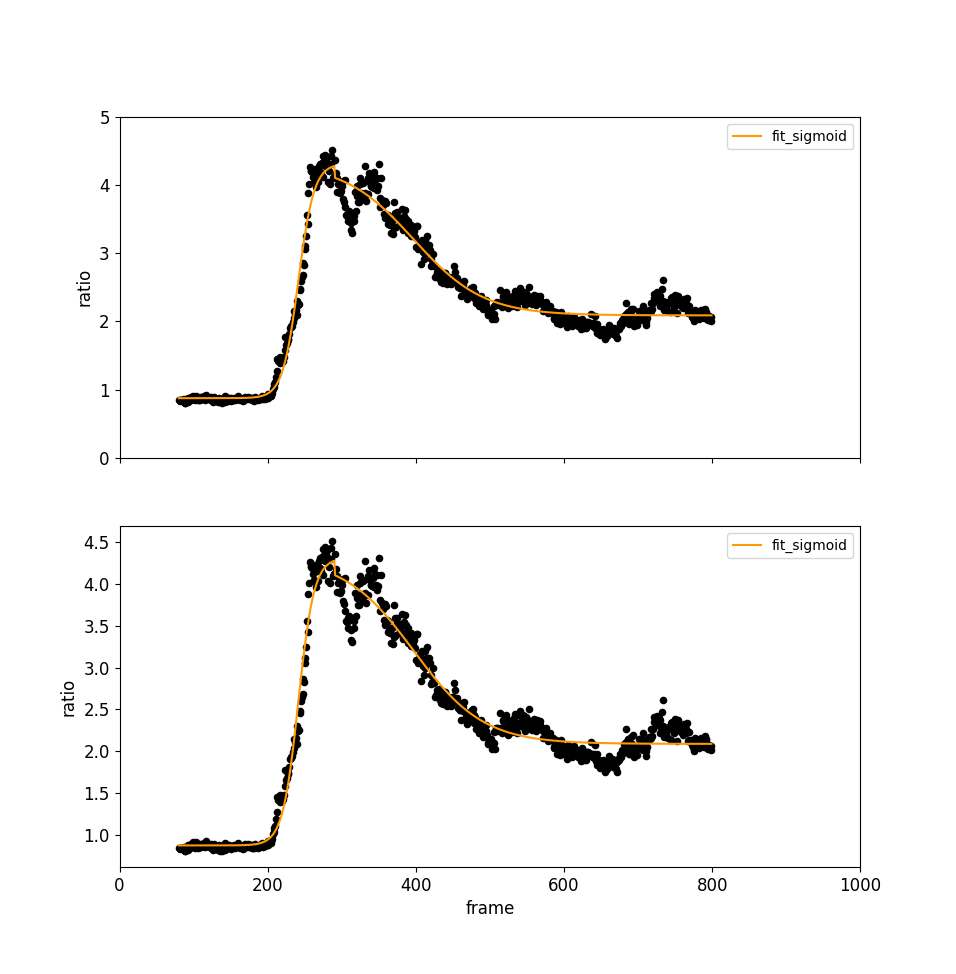
\includegraphics[width=\textwidth]{fig/particle_vis_sigmoid_approx_pos}
	\end{subfigure}
	\hfill
	\begin{subfigure}{0.69\linewidth}
		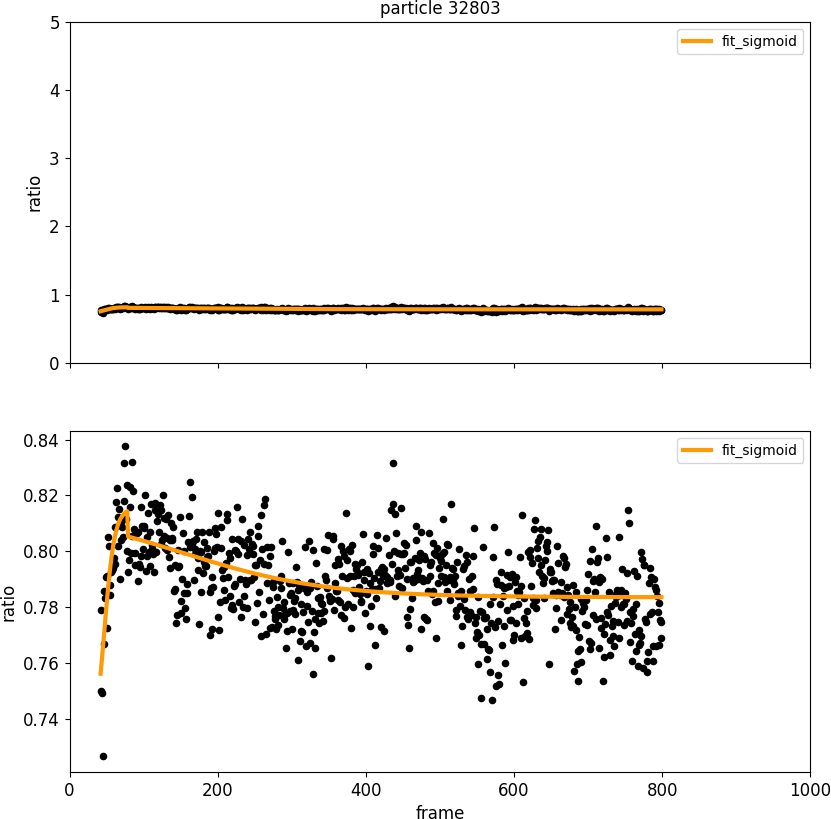
\includegraphics[width=\textwidth]{fig/particle_vis_sigmoid_approx_neg}
	\end{subfigure}
	
	\caption{The upper plot shows the data in black and approximation in orange of an activated cell. The first plot is scaled from 0 to 5, the second one is scaled to fit the data. The lower plot shows the same of an unactivated cell.}
	\label{fig:particle_vis_sigmoid_approx}
\end{figure}

The above-mentioned approximation function is described in pseudocode below.

\begin{algorithm}[H] \label{alg:approximate}
	\SetAlgoLined
	\DontPrintSemicolon
	\LinesNumbered
	\SetKwInOut{Input}{input}
	\SetKwInOut{Output}{output}
	\caption{Approximate}
	
	\Input{particle data as (frame, ratio) matrix}
	\Output{parameters}
	
	\BlankLine
	\Begin{
		set boundaries for parameters\;
		set start values for parameters\;
		use Trust Region Reflective Algorithm with boundaries and start values to get parameters\;
		calculate corresponding approximation and add as fit\_sigmoid columns to data matrix\;
		return paramters\;
	}
\end{algorithm}
\vspace{1cm}

The parameters of $f_{ac}$ used in the approximation are not independent of each other if we choose $t$ to be the point at which $(a-u)/(1+e^{-k_1(x-w_1)})$ almost reaches the value $a$. We choose $t := w_1 - log(1/0.99-1) / k_1 = w_1 - log(1/99) / k_1$ as the function has had $99\%$ of the increase of the sigmoid curve up to this point.

Setting the boundaries in line 2 is non-trivial. We have noted that a condition such as $0 \leq u \leq d \leq a$, $w_1 \leq t \leq w_2$, $k_1 > 0$ and $k_2 < 0$ are expected. We want to impose them using boundaries in which the parameters must lie. However, boundaries for each parameter must not depend on other parameters. We can circumvent this by setting the boundaries as described in table~\ref{tab:boundaries_and_starting_vals}, where we set min val, max val and median val as the minimum, maximum and median of the particles' ratio data respectively while start and end is the first and last frame where data was recorded for this particle. This guarantees

\begin{align*}
	0 \leq \text{min val} \leq u \leq \text{median val} - 0.002 < \text{median val} + 0.002 \leq a \leq \text{max val}\\
	\implies 0 \leq u < a.
\end{align*}

Where $d$ lies within this inequality chain is not fixed. For the condition $w_1 \leq t \leq w_2$ we only guarantee

\begin{align*}
	t = w_1 - \underbrace{\frac{\log(\frac{1}{99})}{k_1}}_{< 0} \geq w_1.
\end{align*}

The other conditions are met as $k_1 \in [0.05, 10] \implies k_1 > 0$ while $k_2 \in [-1, -0.01] \implies k_2 < 0$.

\begin{table}[h!]
	\centering
	\begin{tabular}{|c|c|c|c|}
		\hline
		parameter & lower bound & upper bound & starting value \\ 
		\hline
		$u$ & min val & median val - 0.002 & min val\\
		\hline
		$a$ & median val + 0.002 & max val & max val\\
		\hline
		$d$ & min val & max val & median val\\
		\hline
		$w_1$ & start & end & start\\
		\hline
		$w_2$ & start & end & (start + end) / 2\\
		\hline
		$k_1$ & 0.05 & 10 & 0.1\\
		\hline
		$k_2$ & -1 & -0.01 & -0.03\\
		\hline
	\end{tabular}
	\label{tab:boundaries_and_starting_vals}
	\caption{Upper and lower bounds as well as starting value for each of the independent parameters.}
\end{table}

Starting values can have a big impact on the approximation reached by the algorithm. We want to choose starting values close to the expected resulting parameters. By choosing $w_1$ as the start we favour the first increase in the data to be the point of activation. Otherwise, we are more likely to mistake an oscillation later in the data as the activation point. As we do not know when the activation happens when setting the boundaries we guess that $w_2$ lies in the middle. The other starting values are chosen as we expect $u$ to be low, $a$ to be high, $d$ to lie somewhere in the middle and experimenting showed that $k_1$ often has a value around $0.1$ while $k_2$ lies around $-0.03$.

This work uses the python scipy function \texttt{scipy.optimize.curve\_fit(function, xdata, ydata, p0=starting\_values, method='trf', bounds=(lower\_bounds, upper\_bounds))} as it provides all the necessary functionality. The method parameter \texttt{trf} stands for Trust Region Reflective, as described in section~\ref{subsec:algorithms_bounded_lsp}.

\section{Analysis of the Approximation}

Violin Plots + outliers comparison between activated and unactivated in both human and mouse cells
